\chapter{第1讲：弦理论专题}

\lectureoverview{在\(1+1\)维中，通过玻色化、电--磁对偶、D膜、强耦合相变、涌现几何以及弦真空的组合学景观，对还原论的挑战变得更加尖锐。同一个物理系统可能允许截然不同的基本描述；哪一种描述看起来简单，取决于耦合和几何。}

\section{还原论、复杂性与简单性问题}

Susskind以一个刻意熟悉的哲学口号开场：大的东西由小的东西构成，小的东西由更小的东西构成。随后他补充了同一思想的更具雄心的版本，也就是对基础物理真正重要的那个版本：当人们深入更深的层次时，对象不仅应当变得更小，还应当变得更简单。他的比喻是，房子由砖块构成，而没有人会把房子误认为砖块。砖块更小，但它也更简单。

本讲的第一个动作，是用粒子物理的实际状况来面对这一预期。如果还原论确实在那种强的意义上带来不断增加的简单性，人们或许会期待当今的基本粒子物理已经接近经济。相反，Susskind强调，甚至在量子引力进入之前，账目就已经显得凌乱。在讲座中这些是粗略的计数，但粗略本身正是要点的一部分：
\begin{equation}
\begin{aligned}
N_{\mathrm{species}}&\sim 75,\\
N_{\mathrm{independent}}&\sim 10\text{--}20,\\
N_{\mathrm{parameters}}&\sim 20.
\end{aligned}
\end{equation}
即便如此，事情也还没有结束。标准模型不包含引力，不解释暗物质，不提供暴胀所需的额外结构，并且带有严重的精细调节问题。加入通常的修补机制只会增加计数。超对称就是讲座中的例子。在讲座当时，许多物理学家希望大型强子对撞机会揭示超伴子；Susskind强调，相应的扩展会引入一百多个额外参数，而不是立刻简化账目。他的示意性信息是
\begin{equation}
N_{\mathrm{parameters}}^{\mathrm{extended}} \sim 200.
\end{equation}
这些数字是刻意粗略且具有历史性的。它们服务于这样一个论点：更深的描述在其粒子清单和测量常数的层面上未必看起来更简单。

这一定量上的抱怨还不是Susskind的主要论点。它只是前奏。更深的断言，也是驱动本讲其余部分的断言，是现代量子场论和弦理论并不显然支持一种唯一的、与耦合无关的砖块与房子之分。接下来的例子被选来表明，``基本''这一说法本身的意义可能取决于哪些变量是高效的。

\section{玻色化：固定基本性的第一次破缺}

Susskind的第一个理论例子来自\(1+1\)维量子场论：一维空间，一维时间。他立刻声明，他不会详细推导这一等价性；要点不在于形式证明，而在于概念教训。

人们从费米子的场论出发。费米子场记为\(\psi\)。两个邻近的费米子可以形成一个玻色型复合体，相应的玻色子场记为\(\phi\)。乍看之下，层级似乎很直接：\(\psi\)是基本的，而\(\phi\)是复合的或有效的变量。在讲座中，玻色子正是这样被引入的，作为一个产生费米子束缚对的场。

然而，人们发现同一理论可以从相反的起点重写。人们可以从玻色子场\(\phi\)出发，于是费米子不再作为点状组分出现。相反，它作为玻色子场的一个扭结出现，这是一种延展的构型，其中\(\phi\)在两个渐近值之间平滑地插值。讲座中最小的数学内容是这一渐近结构：
\begin{equation}
\phi(x\to -\infty)=\phi_-,
\qquad
\phi(x\to +\infty)=\phi_+.
\end{equation}
一个方便的示意性代表是
\begin{equation}
\phi(x)\approx \frac{\phi_++\phi_-}{2}
+
\frac{\phi_+-\phi_-}{2}\tanh\!\left(\frac{x}{\ell}\right),
\end{equation}
其中\(\ell\)是过渡区域的宽度。

\editorialnote{双曲正切剖面是讲座中所画扭结的标准光滑代表，而不是在那里推导出的公式。精确的玻色化字典取决于模型；概念要点是费米子激发与玻色子场的拓扑孤子之间的交换。}

讲座中的皮带类比足够精确，值得保留。一条没有扭转的平直皮带，就是没有扭结的构型。如果把一端旋转\(2\pi\)，皮带在远处会回到相同的局部取向，但在中间它必须经过一段延展的扭转区域。那段扭转区域就是扭结。在玻色子描述中，费米子正是由这样一个延展对象来表示的。

一旦引入耦合，这一点就变得更加清晰。Susskind在这个例子中称之为\(G\)。这里要说的并不是两种描述之间有某种模糊的关联，而是两种描述的效率取决于参数区域：
\begin{align}
G \ll 1
&\Rightarrow
\ell\text{ small, tight kink; }\psi\text{ efficient},\\
G \gg 1
&\Rightarrow
\ell\text{ large, broad kink; }\phi\text{ efficient}.
\end{align}
对于小的\(G\)，扭结是紧致的，费米子看起来就像那个简单对象。随着\(G\)增大，扭结变宽，费米子变得不那么像点状。此时玻色子变量就变成更经济的变量。

\paragraph{示意性更新规则。}
\begin{enumerate}
\item 从由\(\psi\)描述的费米子理论出发。
\item 识别由\(\phi\)描述的玻色子复合体。
\item 把同一理论完全用\(\phi\)改写。
\item 在玻色子描述中，费米子作为宽度为\(\ell\)的扭结重新出现。
\item 对于\(G\ll 1\)，\(\ell\)很小，费米子描述最简单。
\item 对于更大的\(G\)，\(\ell\)增大，玻色子描述变得最简单。
\end{enumerate}

这是对固定的``房屋与砖块''图景的第一个明确反例。讲座的要点并不仅仅是复合对象存在，而是什么算作基本变量可以随耦合而改变。

\section{电荷、磁单极子与弱耦合和强耦合}

Susskind接下来问，在更熟悉的粒子物理中是否会出现类似的故事。例子是电荷与磁单极子。一个普通的带电粒子，例如电子，用这种语言来说就是一个电单极子：一个局域化的电场源。磁单极子则通过条形磁铁的类比引入。如果能够以某种方式把条形磁铁的一端分离出来，而不带那根看不见的连接棒，那么场线看起来就会完全像电荷的场线，只不过是磁的而不是电的。

相关的控制参数是精细结构常数\(\alpha\)。在讲座中，Susskind启发式地把它当作电荷的平方：
\begin{equation}
\alpha \sim e^2.
\end{equation}
他还给出了一个粗略的操作性解释：它衡量电子有多容易辐射，并用如下说法概括这一强度：一个加速的电子在相关意义上辐射大约``\(1/100\)''个光子。用讲座自己的粗略数值语言来说，
\begin{equation}
\alpha \approx 10^{-2}.
\end{equation}
这并不是要作为精确约定；它只是一种教学方式，用来编码电荷是弱的这一事实。

\editorialnote{弱--强关系在Dirac量子化中有精确的先例。在一种常见约定中，电荷与磁荷满足\(e g_m=2\pi n\)。因此，弱的电耦合对应于强的磁耦合，尽管精确的数值因子和受保护的质量关系取决于理论。}

当\(\alpha\ll 1\)时，电子是简单对象。它的电场很弱，它的真空极化云很稀薄，它看起来几乎像点状。磁单极子则相反：它的场极其巨大，它的周围被剧烈扭曲，它宽大、复杂且沉重。Susskind正是用这种弱--强的风格概括这一情形：
\begin{equation}
\begin{aligned}
\alpha \ll 1
&\Rightarrow \text{simple electron;}\\
&\phantom{\Rightarrow{}}\text{heavy, extended monopole},\\
\alpha \gg 1
&\Rightarrow \text{simple monopole;}\\
&\phantom{\Rightarrow{}}\text{heavy, structured electron}.
\end{aligned}
\end{equation}
讲座并没有推导单极子质量公式。它也不需要。要点是定性的。随着\(\alpha\)增大，电子的场增强，其结构增大，而单极子则缩小并变轻。远超过1之后，有用的描述发生了交换：单极子变得简单，而电子变得复杂。

这就是早先从玻色化得到的教训的场论版本。基本与复合之间的区分并不是绝对的。它取决于耦合。

\begin{classroomqa}
\audiencequestion{如果还原论不是可靠的指南，为什么物理学家还依赖微积分？微积分似乎把系统分成任意小的部分。\lecturetimestamp{00:21:21}}
\lecturerresponse{微积分断言的是光滑变化；它并不指认理论的基本对象。量子场在每一个距离尺度上涨落，产生无尽的层级，而不是一个最终的、光滑的层次，让人可以在那里一劳永逸地判定什么是基本的。}
\end{classroomqa}

对话继续进行，有人提出这种层级结构类似于分形。Susskind 接受了这个类比，随后将其进一步明确：量子场在每一个尺度上都会涨落，因此在经典意义上从来都不是光滑的。这种过度的变化正是量子场论在数学上困难的部分原因；普通微积分必须用于重整化后的量，而不是用于朴素光滑的微观场。

\section{弦、D-膜与弱--强对偶性的回归}

讲座中的下一个过渡是刻意朴素的。如果弦理论被认为是关于基本构成单元的理论，那么答案肯定很简单：构成单元就是弦。Susskind 公开陈述了这一预期，然后在讲座的下一部分中将其拆解。

\subsection{为什么弦不是故事的全部}

第一个复杂之处是 D-膜不可避免的存在。D\(p\)-膜是一个 \(p\) 维物体，弦可以在其上终止。字母 \(D\) 来自 Dirichlet 边界条件，但名称远不如其作用重要：这些物体是理论的一部分，不能被丢弃。它们不是可选的装饰。

最简单的例子是：
\begin{itemize}
\item 一个 D0-膜，它是点状的，
\item 一个 D1-膜，或 D-弦，它是弦状的，
\item 一个 F-弦，即普通的基本弦。
\end{itemize}
D0-膜是一个重的点状位置，任意数量的 F-弦都可以在其上终止。D1-膜是一个重的缆索状物体，比 F-弦粗得多，单位长度的质量也大得多，但同样是 F-弦可以终止的地方。在弱耦合下，讲座并没有将这些物体呈现为同等基本的替代选项。D-膜被引入为重的、有结构的、看起来像复合物的物体，而理论仍然迫使我们接受它们。

\editorialnote{讲座这一部分所使用的奇膜理论是 IIB 型弦理论。其稳定的 D-膜具有奇数空间维度，包括 D1-膜和 D3-膜。Susskind 推迟给出这些名称，因为当前的主题是对偶性模式，而不是分类学。}

\paragraph{记号。}
Susskind 在讲座的不同部分中 somewhat 宽松地使用 \(G\) 和 \(g\)。这里 \(G\) 保留给玻色化例子，而 \(g\) 表示弦耦合。

弦耦合 \(g\) 是操作性地定义的，而不是公理性地定义的。它是衡量一个涨落弦分裂并形成子弦的概率的参数。这就是为什么 Susskind 直接将其与 QED 中 \(\alpha\) 的作用进行比较。讲座还停下来将张力等同于单位长度的能量：
\begin{equation}
T=\frac{E}{L}=\frac{M}{L}.
\end{equation}

对于 F-弦和 D-弦，标准张力公式使弱--强比较变得明确：
\begin{equation}
T_{\mathrm{F1}}=\frac{1}{2\pi\alpha'},
\qquad
T_{\mathrm{D1}}=\frac{1}{2\pi\alpha' g_s},
\qquad
\frac{T_{\mathrm{D1}}}{T_{\mathrm{F1}}}=\frac{1}{g_s}.
\end{equation}
\editorialnote{这些张力公式提供了讲座中定性的缆索与细线比较背后的常规归一化。它们是编辑添加的；讲座只使用了与耦合的标度关系。}

\subsection{F-弦与 D-弦}

弱--强故事随后在弦的语言中重复自身。在小耦合下，F-弦是轻的、细的，并且接近基本物体最初的直观图像。D-弦是粗的、重的，并且充满了 F-弦结构。随着耦合增大，F-弦更容易分裂；子弦云在其周围增殖，它变得更重、更复杂。与此同时，D-弦越来越难以发射现在很重的 F-弦，因此其周围结构变薄，它变得更轻、更像线。因此讲座的弱--强映射是
\begin{align}
g \ll 1
&\Rightarrow
\begin{gathered}
\text{F-string light and thin;}\\
\text{D-string heavy and structured},
\end{gathered}\\
g \sim 1
&\Rightarrow
\text{F-string and D-string comparable},\\
g \gg 1
&\Rightarrow
\begin{gathered}
\text{D-string light and thin;}\\
\text{F-string heavy and structured}.
\end{gathered}
\end{align}
Susskind 评论说，在 \(g\sim 1\) 附近，这两种描述不再截然不同。超过这一点后，它们实际上交换了角色。这是电子--磁单极子互换的弦论版本，其公认名称是 S-对偶。

同样的交换可以在弦闭合成环之后继续追踪。在弱耦合下，一个小的 F-弦环是轻的类粒子激发，而相应的 D-弦环是重的且复杂的。在强耦合下，它们的角色反转：D-弦环成为轻的描述，而在由此产生的轻闭弦激发中包括引力子。讲座用这个例子坚持认为，即使是一个熟悉粒子的身份，也可能取决于使用对偶性的哪一侧。

讲座把这一点又向前推进了一步。在理想化的理论中，耦合不仅仅是一个可以用手拨动的数字；它表现得像一个场。示意性地，
\begin{equation}
g = g(x).
\end{equation}
因此，空间的不同区域可能偏好不同的对偶描述。在一个区域中，F弦是轻的变量；在另一个区域中，D弦是。在两者之间，没有什么特别简单。这就是为什么对Susskind来说，弦理论并没有恢复简单的还原论图景。它把这种模糊性激进化了。

\editorialnote{在微扰弦理论中，局部耦合由膨胀子设定，\(g_s(x)=e^{\Phi(x)}\)。因此，写下\(g=g(x)\)不仅仅是一个类比，尽管现实的紧化通常会产生一个势，从而约束这类变化。}

\begin{classroomqa}
\audiencequestion{如果耦合变化得足够大，以至于在另一个区域中D弦变得比F弦更轻，这种变化会影响可观测谱吗？\lecturetimestamp{00:34:15}}
\lecturerresponse{会。这正是所讨论的完全对称、数学上受控的模型不能直接等同于我们这个世界的原因之一。它的教益关乎自洽的量子理论能够做什么，而不是自然界的一个字面谱。}
\end{classroomqa}

\begin{classroomqa}
\audiencequestion{对于D2膜，是否存在类似的对偶描述？\lecturetimestamp{00:34:39}}
\lecturerresponse{存在，但它不是另一种类似D弦的交换。偶膜情形将导向膜解释和一个额外的空间维度，这就是下一个构造。}
\end{classroomqa}

\begin{classroomqa}
\audiencequestion{弦分裂的概率更大，是否就解释了内部复杂性的增加？\lecturetimestamp{00:34:53}}
\lecturerresponse{是的。为了使这一机制具体化，回到QED：一个电子发射光子，光子涨落为带电粒子对，而那些带电的线又再次辐射。增大耦合会使这一层级变得不那么稀薄。}
\end{classroomqa}

\subsection{以问题驱动的对量子电动力学的回归}

随后一名学生问，更大的分裂概率是否只是意味着``上游''有更复杂的结构。Susskind通过回到量子电动力学并再次画出电子的世界线来回答。这一回归很重要：它表明弦的故事并不是一个孤立的奇谈，而是同一个弱--强模式的另一个实例。

\begin{figure}[htbp]
\centering
\begin{tikzpicture}[scale=1.0]
\draw[->] (-1.2,0) -- (3.7,0) node[right] {space};
\draw[->] (0,-0.2) -- (0,4.3) node[above] {time};

\draw[line width=0.9pt] (0,0.2) -- (0,4.0);
\node[left] at (0,3.55) {\(e^{-}\)};

\draw[line width=0.8pt] (0,1.0) -- (0.18,1.08) -- (0.36,0.92) -- (0.54,1.10) -- (0.72,0.94) -- (0.90,1.12) -- (1.08,0.96) -- (1.26,1.14);
\draw[line width=0.8pt] (0,2.35) -- (-0.18,2.43) -- (-0.36,2.27) -- (-0.54,2.45) -- (-0.72,2.29) -- (-0.90,2.47);

\draw[line width=0.8pt] (1.26,1.14) -- (1.48,1.42);
\draw[line width=0.8pt] (1.26,1.14) -- (1.04,1.42);
\draw[line width=0.8pt] (1.48,1.42) -- (1.58,2.10);
\draw[line width=0.8pt] (1.04,1.42) -- (0.94,2.10);
\draw[line width=0.8pt] (0.94,2.10) -- (1.58,2.10);

\draw[line width=0.7pt] (1.58,1.78) -- (1.72,1.84) -- (1.86,1.72) -- (2.00,1.86);
\draw[line width=0.7pt] (0.94,1.78) -- (0.80,1.84) -- (0.66,1.72) -- (0.52,1.86);

\node at (2.35,1.95) {\(\gamma\)};
\node at (-1.15,2.75) {\(\gamma\)};
\end{tikzpicture}
\caption{讲座中使用的示意性QED层级：一个点电子发射光子，光子产生粒子对，而子代带电的线又再次辐射，从而在越来越短的尺度上产生结构。}
\end{figure}

讲座的要点是，即使是一个点电子，也伴随着一个过程层级：
\begin{enumerate}
\item 一个电子发射并吸收光子，
\item 一个光子可以产生一个电子--正电子对，
\item 子代带电的线本身也可以发射光子，
\item 这一层级继续延伸到更小的尺度。
\end{enumerate}
对于弱耦合，这团云是稀薄的，因此电子在实验室中看起来几乎像点状。对于更强的耦合，它会增殖，电子就变成一个具有结构的对象。于是，弦的故事被呈现为这一点的直接类比。

同一段后来的讨论也激发了Susskind的启发式能量记账。他坚持认为，相关的能量不仅仅是自由粒子贡献之和。还必须包括相互作用能：
\begin{equation}
E_{\mathrm{tot}} = E_e + E_\gamma + E_{\mathrm{int}}.
\end{equation}
这里\(E_{\mathrm{int}}\)是关键项。正是它使得缀饰电子的质量能够包括与其周围场和虚结构相关的能量。讲座并没有把这变成一次形式化的重整化自能推导。其要点是启发式的，但至关重要：对象的质量已经包括了支撑其周围复杂云所需的相互作用能。

\begin{classroomqa}
\audiencequestion{如果电子没有足够的自由能来产生一个实粒子对，那么虚光子和电子--正电子对的能量从何而来？\lecturetimestamp{00:37:01}}
\lecturerresponse{人们从来不是从一个裸电子开始，然后再附加上它的库仑场。被观测到的电子是一个缀饰态，其质量已经包括了场能和相互作用能。在QED中，总能量并不只是自由电子能量加上自由光子能量；相互作用项是不可或缺的。把中间粒子对称为虚的是有用的，但能量记账属于完整的相互作用态。}
\end{classroomqa}

\begin{classroomqa}
\audiencequestion{当高能探针揭示出这种结构时，究竟是探针创造了它，而不是发现了某种早已存在的东西吗？\lecturetimestamp{00:38:59}}
\lecturerresponse{这种解释上的区分可以争论。从操作层面看，能量足够高的散射具有可计算且非平凡的末态。在弱耦合下，大多数事件看起来仍然简单，而大约有 \(\alpha\) 大小的比例会显示出额外的辐射或粒子对。}
\end{classroomqa}

\begin{classroomqa}
\audiencequestion{当说 D1-膜比 F-弦更重时，它的张力是否也更大？\lecturetimestamp{00:39:37}}
\lecturerresponse{是的。对于延展的弦，这里的``质量''指的是单位长度的能量，而这正是张力。}
\end{classroomqa}

\begin{figure}[htbp]
\centering
\includegraphics[width=0.72\textwidth]{lecture_01_figure_02.png}
\lectureframe{00:38:22.500}

\vspace{1em}

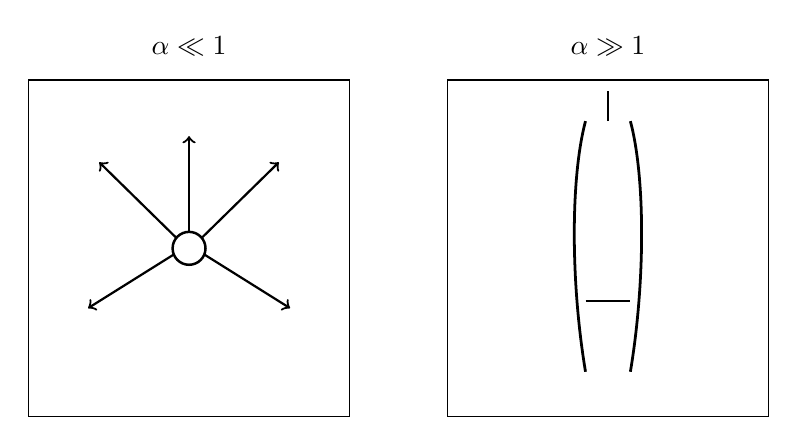
\begin{tikzpicture}[scale=0.95]
\draw (-5.3,-2.4) rectangle (-1.0,2.1);
\draw (0.3,-2.4) rectangle (4.6,2.1);

\node at (-3.15,2.55) {$\alpha \ll 1$};
\node at (2.45,2.55) {$\alpha \gg 1$};

\draw[line width=0.9pt] (-3.15,-0.15) circle (0.22);
\draw[->,line width=0.8pt] (-3.15,0.07) -- (-3.15,1.35);
\draw[->,line width=0.8pt] (-2.98,-0.01) -- (-1.95,1.00);
\draw[->,line width=0.8pt] (-3.32,-0.01) -- (-4.35,1.00);
\draw[->,line width=0.8pt] (-2.95,-0.23) -- (-1.80,-0.95);
\draw[->,line width=0.8pt] (-3.35,-0.23) -- (-4.50,-0.95);

\draw[line width=1.0pt] (2.15,-1.8) .. controls (1.95,-0.6) and (1.95,0.8) .. (2.15,1.55);
\draw[line width=1.0pt] (2.75,-1.8) .. controls (2.95,-0.6) and (2.95,0.8) .. (2.75,1.55);
\draw[line width=0.8pt] (2.15,-0.85) -- (2.75,-0.85);
\draw[line width=0.8pt] (2.45,1.55) -- (2.45,1.95);
\end{tikzpicture}
\caption{在相互作用能量的讨论中，弱--强 QED 比较。该图分离出在 Susskind 附近可见的两个区域：一个稀薄的弱耦合云和一个增殖的强耦合云。}
\end{figure}

尽管弱--强比较此前已经引入，这张图之所以放在这里，是因为在讲座中 Susskind 在这个后来由提问驱动的时刻，在讨论相互作用能量和增殖结构时重新绘制了这一对比。

\section{偶膜理论与涌现的额外维度}

至此，讲座一直在讲述一个关于交换的强有力故事：费米子对玻色子、电子对磁单极子、F-弦对 D-弦。下一步更加令人惊讶。Susskind 转向弦理论的另一个版本，其中使用的是偶数维 D-膜，而不是奇数维的。这一区别很重要，因为在这个理论中没有可与 F-弦交换的 D-弦。人们有 D0-膜、D2-膜、D4-膜，等等。

因此，强耦合极限不能简单地把一种弦重新标记为另一种弦。根据讲座，会发生更奇怪的事情：一个额外的空间维度变得显明。Susskind 故意先以最戏剧化的形式陈述这一点 --- ``一个新维度实体化'' ---，然后立即将其转化为更谨慎的陈述：一个非常小的紧致方向膨胀到不再能被忽略。

这种记账本身就是要点的一部分，因此他对此稍作停顿：
\begin{equation}
\begin{aligned}
10\text{-dimensional string theory} &= 9\text{ space}+1\text{ time},\\
11\text{-dimensional theory} &= 10\text{ space}+1\text{ time}.
\end{aligned}
\end{equation}
讲座的主张是，偶膜理论的强耦合极限实际上是十一维的。

\editorialnote{偶膜理论就是 Type IIA 弦理论，其强耦合完备化是 M-理论。在标准单位中，涌现圆的半径和十一维普朗克长度按 \(R_{11}=g_s\ell_s\) 和 \(\ell_{11}=g_s^{1/3}\ell_s\) 标度。这些名称和公式明确给出了讲座几何叙述背后的现代词典。}

\subsection{花生酱三明治}

为了描绘紧致方向，Susskind 使用了``花生酱三明治''模型：两片无限薄的面包，中间是真实空间。特殊规则是，从一侧出去会回到另一侧。用讲座以图示而非形式方式描述的一种常规记号，可以写为
\begin{equation}
y \sim y + 2\pi R.
\end{equation}
如果 \(R\) 非常小，生活在三明治中的观察者实际上会把他们的世界描述为低维的。关键的强耦合更新则是
\begin{equation}
g\uparrow
\qquad \Longrightarrow \qquad
R_{\mathrm{compact}}\uparrow.
\end{equation}
这就是 Susskind 说一个新的空间维度出现时的意思：并不是空间从无中被创造出来，而是一个先前很小的紧致方向膨胀，并在有效理论中变得可见。

\begin{figure}[htbp]
\centering
\resizebox{\linewidth}{!}{%
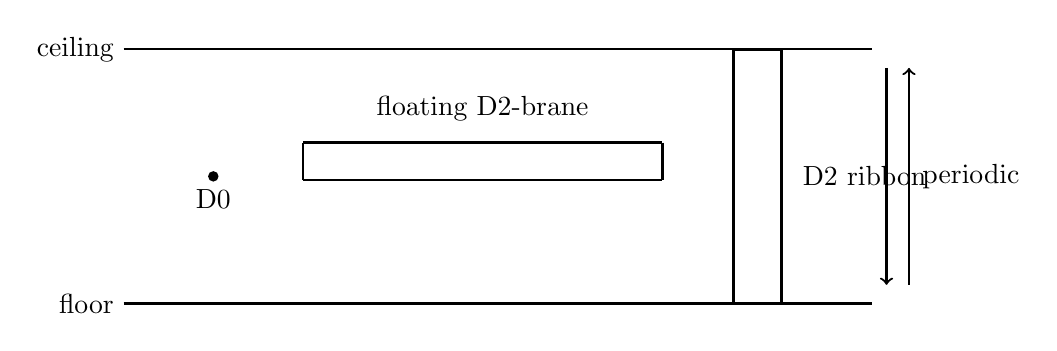
\begin{tikzpicture}[scale=0.95]
\draw[line width=0.9pt] (-5,1.7) -- (5,1.7);
\draw[line width=0.9pt] (-5,-1.7) -- (5,-1.7);

\node[left] at (-5,1.7) {ceiling};
\node[left] at (-5,-1.7) {floor};

\draw[->,line width=0.8pt] (5.2,1.45) -- (5.2,-1.45);
\draw[->,line width=0.8pt] (5.5,-1.45) -- (5.5,1.45);
\node[right] at (5.55,0) {periodic};

\draw[line width=1.0pt] (-2.6,0.45) -- (2.2,0.45);
\draw[line width=1.0pt] (-2.6,-0.05) -- (2.2,-0.05);
\draw[line width=1.0pt] (-2.6,0.45) -- (-2.6,-0.05);
\draw[line width=1.0pt] (2.2,0.45) -- (2.2,-0.05);
\node at (-0.2,0.9) {floating D2-brane};

\draw[line width=1.0pt] (3.15,-1.7) -- (3.8,-1.7);
\draw[line width=1.0pt] (3.15,1.7) -- (3.8,1.7);
\draw[line width=1.0pt] (3.15,-1.7) -- (3.15,1.7);
\draw[line width=1.0pt] (3.8,-1.7) -- (3.8,1.7);
\node[right] at (3.95,0) {D2 ribbon};

\fill (-3.8,0) circle (0.07);
\node[below] at (-3.8,-0.05) {D0};
\end{tikzpicture}
}%
\caption{三明治紧致化。上下边界被周期性地认同；一个 D2-膜像地毯一样漂浮在它们之间，而另一个从地板延伸到天花板，当紧致方向很小时看起来像弦。}
\end{figure}

\subsection{D0-膜和 D2-膜会变成什么？}

讲座现在问 D0-膜和弦会发生什么。答案是不对称的。当 \(g\) 变大时，D0-膜变得越来越轻；在更高维解释中，它们加入携带新显明方向动量的粒子塔。因此，弱耦合图像中一个沉重而复杂的物体，在强耦合图像中变成了普通的轻激发。

质量关系式给出了这一等同：
\begin{equation}
M_{D0}(n)=\frac{n}{g_s\ell_s}
=\frac{n}{R_{11}}
=M_{\mathrm{KK}}(n).
\end{equation}
\editorialnote{Susskind 把 D0-膜称为十一维理论中的``引力子''。更确切地说，它们的束缚态是十一维超引力多重态的 Kaluza--Klein 动量模式，而该多重态的无质量部分包含引力子。这一区分既保留了讲座中的物理等同，又避免了字面上把单个粒子说得过头的表述。}

D2-膜解释了弦的命运。讲座中强调了两种构型：
\begin{enumerate}
\item 一张 D2-膜像花生酱中的地毯一样漂浮在地板和天花板之间；
\item 一张 D2-膜像丝带一样从地板拉伸到天花板，沿着可见方向延展。
\end{enumerate}
当三明治很薄时，这条丝带看起来实际上是二维的。它就是低能观测者所称的弦。随着紧致方向展开，同一个物体就变得毫无疑问地像膜了。由于它现在在竖直方向上包含更多物质，它变得很重，不再像弦。

\paragraph{转变的逻辑。}
\begin{enumerate}
\item 从一个非常薄的紧致方向开始，于是从地板到天花板的丝带实际上表现得像一根弦。
\item 增大 \(g\)，紧致方向随之膨胀。
\item D0-膜变得很轻，并被重新解释为高维理论中的 Kaluza--Klein 动量态。
\item 像弦一样的 D2 丝带变成明显延展的膜，并变得很重。
\end{enumerate}
这就是讲座从对偶性转向涌现几何的枢纽。强耦合并不只是把一个物体换成另一个物体；它改变了哪一种几何才是有效的。

Susskind 停下来思考这听起来有多么奇怪。所提出的等同关系网需要困难的数学一致性关系，其中一些最初以猜想的形式出现在物理学家面前，后来才由数学家确立。他的主张并不是每一个现实的弦真空都已被理解，而是对偶关系网本身经受住了异常严格的检验。

在这个理想化设定中，如果耦合逐处变化，那么有效几何也会随之变化。一个区域可能看起来几乎是十维的，其中有轻的弦和重的 D0-膜；另一个区域则可能展开为十一维描述，其中有重的包裹膜和轻的 Kaluza--Klein 模式。这种局部的语言变化是对偶关系网的一部分。

文字记录一度把这些关系称为``不等式''。在上下文中，本意是\emph{对偶性}：参数空间两端之间的关系。这一更正很重要，因为讲座的结论恰恰是：并不存在已知的唯一基本组分清单。弦、膜、粒子以及高维几何可以相互转化；要么关系网中没有任何成员是绝对基本的，要么某种更深层的组织方式仍然未知。

\section{D3-膜、包裹膜与对偶性的几何图像}

休息之后，Susskind 明确地把这个主题描述为一个由相互关联的理论和思想构成的``巨大关系网''。接下来的例子并不是新的孤立效应；它们是把先前的例子联系起来的桥梁。

\subsection{D3-膜的世界体积}

第一座桥梁使用 D3-膜。一张 D3-膜有三个空间维度，被限制在其中的观测者很容易把它误认为普通空间。膜可以弯曲和涨落，而终止于其上的弦可以连接、分裂和散射。对于只看到沿膜方向的观测者来说，每个端点看起来像一个粒子，而端点之间的相互作用看起来像普通的量子场论。

\begin{figure}[htbp]
\centering
\resizebox{\linewidth}{!}{%
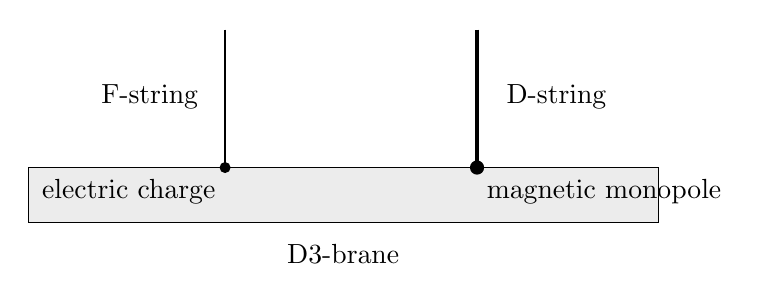
\begin{tikzpicture}[scale=1.0]
\draw[fill=gray!15] (-4,-0.35) rectangle (4,0.35);
\node at (0,-0.75) {D3-brane};

\draw[line width=0.9pt] (-1.5,2.1) -- (-1.5,0.35);
\fill (-1.5,0.35) circle (0.07);
\node[left] at (-1.72,1.25) {F-string};
\node[below left] at (-1.5,0.32) {electric charge};

\draw[line width=1.5pt] (1.7,2.1) -- (1.7,0.35);
\fill (1.7,0.35) circle (0.09);
\node[right] at (1.95,1.25) {D-string};
\node[below right] at (1.7,0.32) {magnetic monopole};
\end{tikzpicture}
}%
\caption{D3-膜世界体积解释。F 弦的端点表现为电荷；D 弦的端点表现为磁单极子。}
\end{figure}

这是讲座中最令人满意的等同之一。终止于 D3-膜上的 F 弦在世界体积观测者看来是电荷。终止于同一张膜上的 D 弦则表现为磁单极子。换句话说，F 弦与 D 弦之间的对偶性，在 D3-膜世界体积上变成了普通场论的电--磁对偶性。先前只是类比的东西，现在成了一份明确的词典。

\editorialnote{对于一叠D3膜，低能世界体描述是四维\(\mathcal N=4\)超对称Yang--Mills理论。其电--磁对偶是IIB型S对偶的场论实现；单张膜给出讲座中图示所用的阿贝尔极限。}

\subsection{两个紧致方向与非对称缠绕}

Susskind随后回到高维几何，并紧致化不止一个而是两个小方向。由于无法在黑板上画出十一维，他将草图中未用到的七个大方向压缩为一个可见的水平方向，然后明确画出两个紧致方向。他坚持非对称地画出紧致化，因为若要使有效弦具有不同的张力，一个紧致方向必须比另一个更短。

\begin{figure}[htbp]
\centering
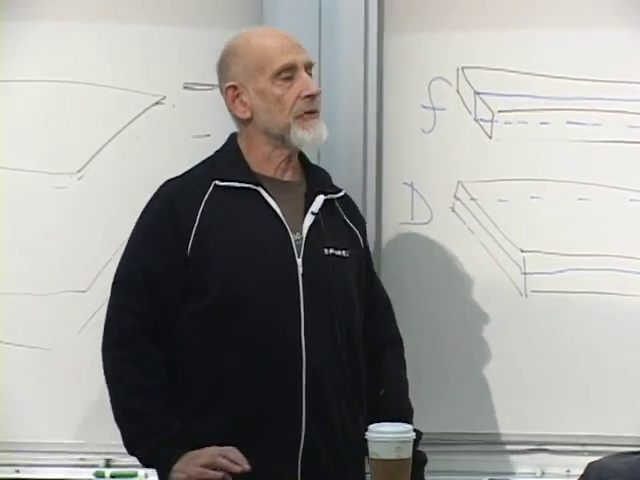
\includegraphics[width=0.78\textwidth]{lecture_01_figure_03.png}
\lectureframe{01:10:25.000}
\caption{两个缠绕膜的完整黑板状态。短与长的紧致循环产生右侧画出的类F弦与类D弦的带状结构。}
\end{figure}

一张膜可以缠绕任一紧致方向，并从非紧致方向看像一根弦。若\(R_1\)与\(R_2\)是两个圆的半径，则其有效张力为
\begin{equation}
\begin{aligned}
T_{(1)}&=2\pi R_1 T_{\mathrm{M2}},\\
T_{(2)}&=2\pi R_2 T_{\mathrm{M2}},\\
\frac{T_{(1)}}{T_{(2)}}&=\frac{R_1}{R_2}.
\end{aligned}
\end{equation}
因此不相等的圆尺寸产生不相等的弦张力。将较短的缠绕认定为轻的F弦、较长的认定为重的D弦，可以示意性地写出
\begin{equation}
g_s\sim \frac{R_{\mathrm{short}}}{R_{\mathrm{long}}},
\qquad
\frac{T_{\mathrm{D1}}}{T_{\mathrm{F1}}}\sim \frac{1}{g_s}.
\end{equation}

\begin{classroomqa}
\audiencequestion{这幅图像中的耦合能否理解为两个紧致维度之比？\lecturetimestamp{01:10:13}}
\lecturerresponse{可以。弱--强参数被几何化为一个纵横比。使一个方向变短会产生小耦合；交换两个方向则交换轻弦与重弦。}
\end{classroomqa}

\editorialnote{讲座暂时将这个比值称为\(\alpha\)，沿用了此前用于QED精细结构常数的符号。我们在此写作\(g_s\)，以保持两种含义彼此区分。在完整的M理论构造中，IIB型耦合被编码在紧致二维环面的复结构中；精确的分子取决于其循环如何标记。}

缠绕膜图像可以在不带有黑板绘图透视畸变的情况下加以概括：

\begin{figure}[htbp]
\centering
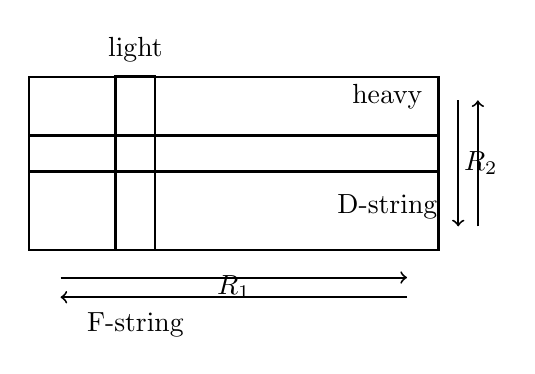
\begin{tikzpicture}[scale=1.0]
\draw[line width=0.9pt] (0,0) rectangle (5.2,2.2);
\node[below] at (2.6,-0.2) {\(R_1\)};
\node[right] at (5.4,1.1) {\(R_2\)};

\draw[->,line width=0.7pt] (5.45,1.9) -- (5.45,0.3);
\draw[->,line width=0.7pt] (5.7,0.3) -- (5.7,1.9);
\draw[->,line width=0.7pt] (0.4,-0.35) -- (4.8,-0.35);
\draw[->,line width=0.7pt] (4.8,-0.6) -- (0.4,-0.6);

\draw[line width=1.0pt] (1.1,0) -- (1.6,0) -- (1.6,2.2) -- (1.1,2.2) -- cycle;
\node at (1.35,2.55) {light};

\draw[line width=1.0pt] (0,1.45) -- (5.2,1.45);
\draw[line width=1.0pt] (0,1.00) -- (5.2,1.00);
\node at (4.55,1.95) {heavy};

\node at (1.35,-0.95) {F-string};
\node at (4.55,0.55) {D-string};
\end{tikzpicture}
\caption{两种缠绕膜构型从非紧致方向看都像弦，但不相等的紧致尺度使一根有效弦比另一根更轻。}
\end{figure}

这是早先对偶故事的几何版本。挤压一个方向同时拉伸另一个方向，会使一个缠绕对象更重而另一个更轻，因此F弦与D弦的角色可以互换。

\begin{classroomqa}
\audiencequestion{如果紧致方向是循环的，那么缠绕对象是否无限宽？\lecturetimestamp{01:10:41}}
\lecturerresponse{不是。紧致圆具有有限周长，即使可以反复绕行而不会到达边缘。剖开绘图的顶部与底部代表同一个点，正如区间的端点可以代表一个圆上的同一点。}
\end{classroomqa}

\begin{figure}[htbp]
\centering
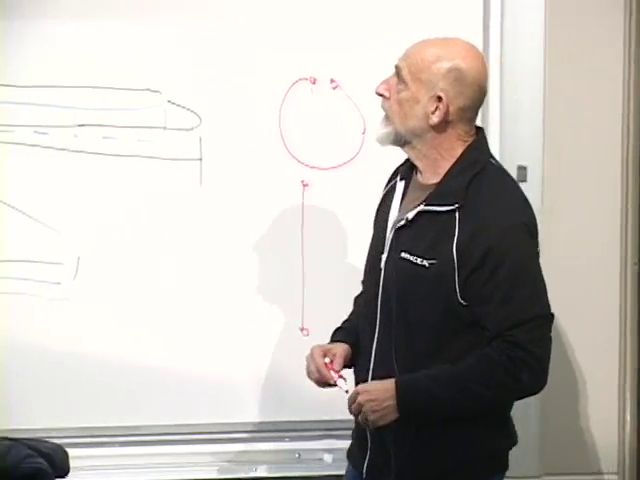
\includegraphics[width=0.78\textwidth]{lecture_01_figure_04.png}
\lectureframe{01:12:25.000}

\vspace{1em}

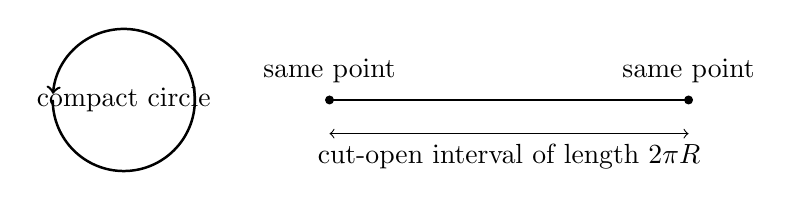
\begin{tikzpicture}[scale=0.95]
\draw[line width=0.9pt,->] (-3.7,0) arc[start angle=180,end angle=535,radius=0.95];
\node at (-2.75,0) {compact circle};
\draw[line width=0.9pt] (0.0,0) -- (4.8,0);
\fill (0.0,0) circle (0.06);
\fill (4.8,0) circle (0.06);
\draw[<->] (0.0,-0.45) -- (4.8,-0.45);
\node at (2.4,-0.75) {cut-open interval of length \(2\pi R\)};
\node[above] at (0.0,0.1) {same point};
\node[above] at (4.8,0.1) {same point};
\end{tikzpicture}
\caption{紧致圆及其剖开后的黑板表示。穿过一个端点会从另一个端点返回；若沿圆运动的同时也沿非紧致方向运动，则会描出一条螺旋线。}
\end{figure}

\begin{classroomqa}
\audiencequestion{为什么紧致路径是圆而不是螺旋线？\lecturetimestamp{01:12:23}}
\lecturerresponse{在非紧致方向的每个固定点处，紧致方向都是一个圆。只有当沿非紧致方向前进的同时又绕圆缠绕时，才会出现螺旋线。黑板上的区间只是把一个圆剖开，其两个端点被等同。}
\end{classroomqa}

\begin{classroomqa}
\audiencequestion{这种几何本身能否解释D膜在被近距离探测时如何看起来像一组F弦？\lecturetimestamp{01:12:49}}
\lecturerresponse{联系是存在的，但在这个初等图像中并不显然；要看出它需要更多几何工具。该图意在组织对偶，而不是推导每一个微观组成描述。}
\end{classroomqa}

\begin{classroomqa}
\audiencequestion{当在空间中移动或随时间演化时，长与短的紧致方向能否交换？\lecturetimestamp{01:13:35}}
\lecturerresponse{在理想化模型中两者皆可。压扁一个循环同时膨胀另一个循环，会交换哪根缠绕弦是轻的。这是``基本弦''只是一个名称的另一个原因：偏好的描述可以随区域或随时间而改变。}
\end{classroomqa}

\section{理想化、特殊对称点与景观}

讲座的最后一部分从优雅的对偶性例子退后一步，追问它们对真实世界说明了什么、又没有说明什么。

首先，Susskind 警告说，那些被精确控制的对偶性，是高度理想化的超对称理论的特征；在这些理论中，玻色子和费米子以完全匹配的质量出现。他将其类比为牛顿力学中的圆轨道：人们首先研究它们，是因为它们对称且数学上易于处理，而不是因为实际的行星运动可以被完美的圆穷尽。完全同样地，超对称弦理论之所以更容易分析，是因为它们比自然所显现的更为对称。

尽管如此，这种理想化仍具有启发性。一个完美的圆轨道并不是一个现实的行星系统，但它展示了在对称性较低的轨道中仍然存留的特征。同样地，超对称例子展示了量子力学、引力和微观结构能够相互协调的若干自洽方式。Susskind 刻意给出的尖锐表述是：那些易于处理的弦理论，字面上并不是关于我们世界的理论；它们的价值在于揭示了很可能在对称性较低、也更难以处理的情形中重新出现的现象。

\subsection{一个可产生许多结果的构造套件}

D-膜只是可用构造套件的一部分。讲座还提到了通量、轨形和定向轨形。人们首先选择一个紧致几何，然后选择哪些膜和通量占据它的循环。即便是简单的三明治结构，当插入一个漂浮的 D2-膜、两个或三个时，其低维物理也会发生变化。增加或减少这类成分会改变有效粒子、相互作用和参数。

假设，按照讲座的示意性计数，一个六维紧致空间大约有 \(500\) 个循环，而每个循环允许大约 \(10\) 种包裹膜、通量或相关结构的选择。那么构造的数目就像下式那样增长：
\begin{equation}
N_{\mathrm{vacua}} \sim 10^{500}.
\end{equation}
讲座的计数逻辑是初等的：
\begin{equation}
10 \times 10 \times \cdots \times 10 = 10^{500}
\end{equation}
其中有 \(500\) 个因子。DNA 类比以更熟悉的语域表达了同一点：
\begin{equation}
N_{\mathrm{DNA}}(500)=4^{500}.
\end{equation}
在 DNA 比较过程中，一位听众确认一条链上有四种选择：A、C、G 和 T。这一更正强化而非改变了论证。一份简短的局部选择清单，重复许多次，就会产生数量庞大的整体排列。确切的指数并不是重点，Susskind 称 \(10^{500}\) 是一个过时的低估；重点在于组合式的增殖。

这给出了对开头还原论期望的最终反转。复杂的粒子物理未必来自复杂的微观规则。它可能之所以出现，是因为我们的真空是许多简单成分的一种复杂排列，正如一个复杂的生物体可以由四种碱基构成的序列编码。

\begin{classroomqa}
\audiencequestion{在把由对偶性联系起来的等价描述等同之后，完整信息是否会只选出这些可能真空中的一个或少数几个，作为对我们世界的描述？\lecturetimestamp{01:26:11}}
\lecturerresponse{想必它会选出一个受限的集合，但许多不同的真空在可及能量下可能看起来极其相似。所引用的景观数目，其本意是在对偶描述被等同之后仍然很大，而不相关的高能细节可能起到像 ``垃圾 DNA 那样的作用。''}
\end{classroomqa}

\subsection{对称点与一般复杂性}

在景观之内存在特别对称的点。在几何图像中，一个等宽高比构型
\begin{equation}
R_1=R_2,
\end{equation}
使两种包裹描述同样简单。在电--磁类比中，这被示意性地表示为
\begin{equation}
m_{\mathrm{monopole}}=m_e.
\end{equation}

\begin{figure}[htbp]
\centering
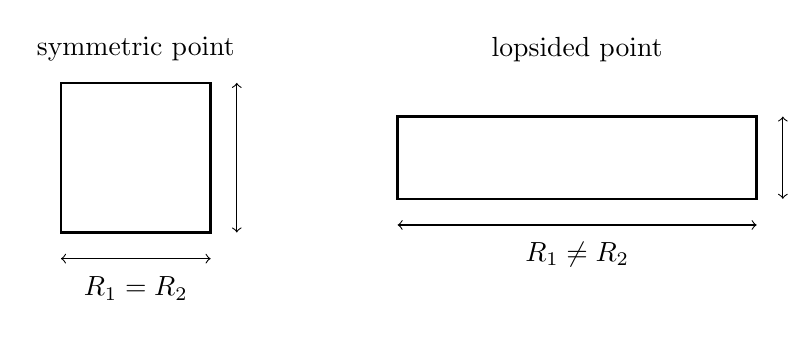
\begin{tikzpicture}[scale=0.95]
\draw[line width=0.9pt] (-4.5,-1.0) rectangle (-2.5,1.0);
\draw[<->] (-4.5,-1.35) -- (-2.5,-1.35);
\draw[<->] (-2.15,-1.0) -- (-2.15,1.0);
\node at (-3.5,1.45) {symmetric point};
\node at (-3.5,-1.75) {$R_1=R_2$};

\draw[line width=0.9pt] (0.0,-0.55) rectangle (4.8,0.55);
\draw[<->] (0.0,-0.9) -- (4.8,-0.9);
\draw[<->] (5.15,-0.55) -- (5.15,0.55);
\node at (2.4,1.45) {lopsided point};
\node at (2.4,-1.3) {$R_1\ne R_2$};
\end{tikzpicture}
\caption{等宽高比的紧致化对称地对待两种包裹弦；而偏斜的紧致化使一种描述比另一种轻得多。}
\end{figure}

\begin{classroomqa}
\audiencequestion{景观中是否存在这样的真空：由于 F-弦和 D-弦描述重合，构造变得简单得多？\lecturetimestamp{01:27:21}}
\lecturerresponse{是的，存在特别对称的点。我们的世界似乎并不位于其中之一：熟悉的电粒子和磁单极子并不具有相等的质量。自然为何占据一个偏斜的点，尚不清楚。}
\end{classroomqa}

\editorialnote{电子--单极子质量相等，是一个受到适当保护的自对偶模型的示意性特征，而不是普通非超对称 QED 的预言。它表达的是讲座的对称点思想，而不是关于观测到的电子的断言。}

萨斯坎德随后回顾了通信理论中的一个类比。随机码可以极其出色，而最容易描述和解码的码则带有额外的数学结构，历史上表现反而不那么好。编码理论后来找到了极为有效的结构化构造，但这个类比依然成立：任何能被简洁命名或描述的东西，都占据着全部可能性空间中一个非常特殊、低复杂度的角落。同样，最容易计算的弦真空可能也是非典型的简单情形。

因此，恰当的问题可能会发生变化。与其要求给出每一个微观细节上的精确紧化，人们可以转而追问哪些特征在广泛的系综中是共同的或普遍的。萨斯坎德将此作为一个研究问题提出，而非已定的结论，并且拒绝以意识形态论证取代计算。

\subsection{宇宙学问题}

\begin{classroomqa}
\audiencequestion{一个周长极大的紧致方向与一个无限方向在观测上有区别吗？我们是否知道我们的三个大空间维度是无限的？\lecturetimestamp{01:30:03}}
\lecturerresponse{我们并不知道它们是无限的。一个闭合的三维球面可以在保持紧致的同时膨胀。对近平坦性的测量只给出曲率半径的下界，正如测量一片近乎平坦的田地可以限定地球的大小，却不能证明其表面是无限的。只有探测到曲率或整体认同，才能确定有限的尺度。}
\end{classroomqa}

\begin{classroomqa}
\audiencequestion{如果在理想化模型中耦合可以随空间变化，那么这种变化在现实世界中如何发生？\lecturetimestamp{01:32:43}}
\lecturerresponse{并不是像对称性示例中所用的那种不受限制的光滑变化。稍后将讨论的现实可能性，是通过具有不同有效定律的区域之间的离散跃迁来实现变化。这种跃迁是否发生是一个宇宙学问题。}
\end{classroomqa}

\editorialnote{这一回应应被理解为讲座对通量真空和畴跃迁的预告，而不是禁止一切光滑变化的标量场的一般定理。观测强烈限制无量纲耦合的变化，而稳定化机制则决定在给定模型中是否仍有连续的模可用。}

录音没有保留最后一位听众的提问。留存下来的回应说，所提出的现象对某些类型的黑洞可以发生，但不会发生在普通施瓦西黑洞的视界处，因为对自由下落的观测者而言，该视界局部上是一个普通的地方。由于问题无法可靠地复原，不再将更具体的论断归于这次交流。

\section{从砖块到描述之网}

认为物理学的更深层次必定更简单的希望已被证明是脆弱的。在\(1+1\)维玻色化中，同一理论既可以围绕费米子组织，也可以围绕玻色子组织，而费米子则作为扭结重新出现。在量子电动力学中，弱耦合与强耦合交换了电子与磁单极子的描述角色。在弦理论中，F弦与D弦重复了同样的模式，而在偶膜理论中，强耦合走得更远：一个紧致方向膨胀，D0膜变成Kaluza--Klein动量态，有效弦被重新解释为更高维几何中包裹的膜。因此，现代量子场论和弦理论并没有为``哪些是砖块，哪些是房屋？''这一问题提供唯一的、一劳永逸的答案。它们提供的是一张描述之网，每一种描述在各自的适用范围内都是高效的，同时还伴随着一个巨大的可能构造的景观，其普遍产物是复杂性而非简单性。
